\chapter{Dangless -- Implementation}
\label{ch:implementation}

\section{Overview}

Dangless is a drop-in replacement memory allocator that provides a custom implementation of the standard C memory management functions \lstinline!malloc()!, \lstinline!calloc()!, \lstinline!realloc()!, \lstinline!free()! and a few others. It aims to solve the problems that dangling pointers lead to by guaranteeing that any access through a dangling pointer will fail, and the application will terminate. It relies on the underlying memory allocator to perform the actual allocation and deallocation. In principle, because Dangless makes no assumptions on the nature or behaviour of the underlying allocator -- referred to as "system allocator" by Dangless --, it should be usable on top of even non-standard implementations such as Google tcmalloc~\cite{google-tcmalloc}.

Catching dangling pointer accesses is ensured by \emph{permanently} marking memory regions as no longer in use upon deallocation (e.g. a call to \lstinline!free()!). Therefore, during the lifetime of the application, in principle, no other memory will be allocated in such a way that it would visibly alias a previously used location: see Figure~\ref{fig:dangless_simplified}.

\begin{figure}
	\centering
	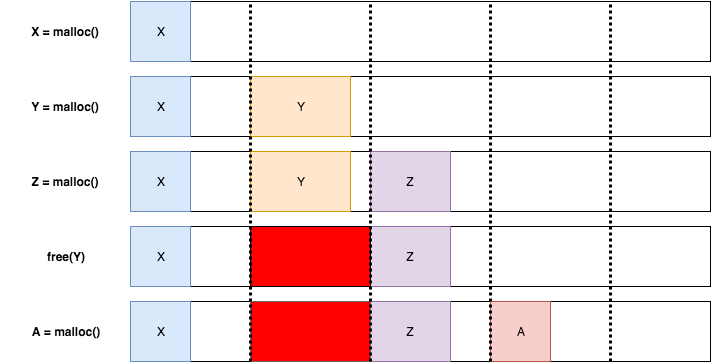
\includegraphics[width=\textwidth]{img/dangless_simplified.png}
	\caption{A simplified view of the virtual memory address space when using Dangless: memory pages are never re-used.}
	\label{fig:dangless_simplified}
\end{figure}

Of course, the physical memory available is very limited even on modern systems, and not re-using is hopeless. The trick then, is to leave the management of physical memory to the system allocator, and change how the physical allocations are mapped to virtual memory: the address space that user applications interact with.

Since we want to rely on the system allocator to efficiently manage physical memory, instead of hijacking the pointer it returns following a successful allocation, we rather \emph{re-map} the physical memory region into a new virtual memory region that's entirely controlled by us. This means that the same allocation will be visible at two virtual memory addresses: the canonical address, managed by the system allocator but not returned to the user code; and the remapped address, managed by Dangless. Note that this re-mapping occurs on the page level (as all virtual memory management has to be), leading to each allocation using up at least one virtual memory page, even if it's smaller than that. See Figure~\ref{fig:dangless_virtremap_mappings} and Figure~\ref{fig:dangless_virtremap_view}. A detailed explanation of these diagrams will follow in Section~\ref{ssec:remapping}.

\begin{figure}
	\centering
	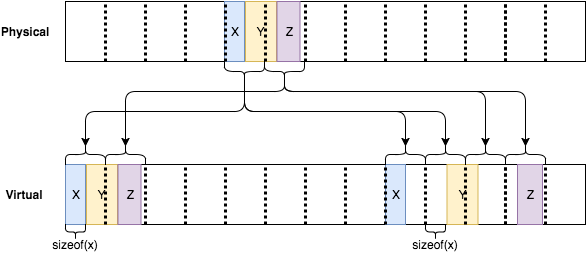
\includegraphics[width=\textwidth]{img/dangless_virtremap_mappings_xyz.png}
	\caption{Remapping the same physical memory region into a new virtual memory region: the same allocation will be visible in virtual memory at two addresses.}
	\label{fig:dangless_virtremap_mappings}
\end{figure}

\begin{figure}
	\centering
	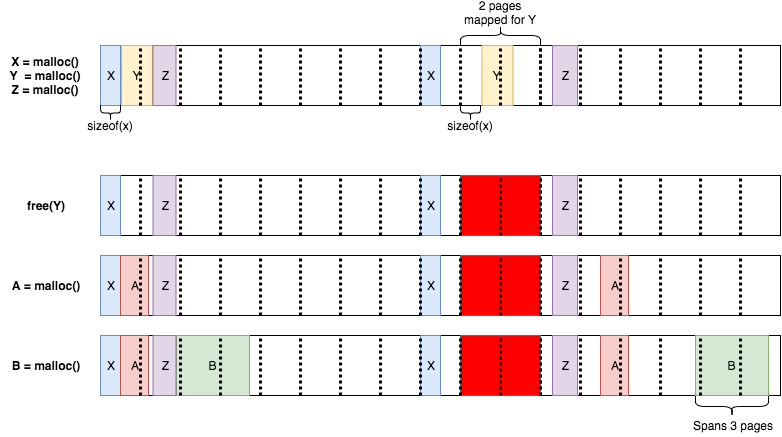
\includegraphics[width=\textwidth]{img/dangless_virtremap.png}
	\caption{View of the virtual memory with Dangless remapping allocations}
	\label{fig:dangless_virtremap_view}
\end{figure}

Virtual memory is plentiful: on the x86-64 architecture, pointers are 64-bit long, which in theory means $2^{64}$ bytes of addressable memory. In practice however, on all current processors that use this architecture, only 48 bits are used, which limits the size of the address space we can work with to $2^{48}$ bytes, or 256 terrabytes. That's also not unlimited, but in practice it's close enough to be sufficient. \todo{Need to elaborate on this somewhere, or cite}

Normally, the difference between physical and virtual memory is entirely hidden from the user code, and is dealt with only by the operating system kernel. This allows the overwhelming majority of users and developers - even programmers working with lower-level languages such as C++ - to work and develop software without ever being aware of the difference, while enjoying the benefits of it. The Linux kernel does provide some system calls that allow the virtual memory to be manipulated, notably \lstinline!mprotect()! which is used to manage access permissions (readable, writeable, executable) of memory regions. This is useful for example when developing just-in-time (JIT) compilers such as the ones employed by browsers to run JavaScript code. Another example is \lstinline!mremap()!, which allows a memory region to be moved almost for free, an ability that makes it useful for garbage collectors for instance. Of course,  \lstinline!mmap()! and \lstinline!munmap()! also primarily work by manipulating virtual memory mappings.

These system calls are sufficient to implement the functionality of Dangless, with some caveats -- in fact, this is exactly how tools like Oscar operate, as discussed in Related Work~\ref{sec:related-work}. The biggest issue is that of performance: system calls are expensive compared to normal memory allocations, and in this scheme, for every single memory allocation, at least one extra system call would be required. The costs and possibilities for optimizations are explored in depth by the Oscar paper.

% The solution Dangless uses is a technology called Dune \todo{reference}: a Linux kernel module and library that provides a lightweight virtualization layer based on Intel VT-x. Using Dune, a normal Linux application can choose to enter a virtualized environment where it has ring-0 privileges, allowing it to efficiently and directly manipulate virtual memory mappings and the interrupt descriptor table, while retaining the ability to perform system calls on the host kernel using the \lstinline!vmcall! instruction. In principle, an application running in Dune mode has the best of both worlds; normal Linux libraries and executables are able to run in Dune mode without any modifications, while gaining access to ring-0 features when beneficial. While there is an overhead associated with running in a virtualized environment, especially when performing \lstinline!vmcall!s, in practice this turns out to be negligible for most applications.

\section{Initialization}
\label{sec:dangless-init}

Dangless has to be initialized before any memory allocation is performed, otherwise those allocations will not be protected. The \lstinline!REGISTER_PREINIT! option, enabled by default, controls whether Dangless should automatically register its initialization function (\lstinline!dangless_init()!) to the \lstinline!.preinit_array! section of the executable, to be called automatically during start-up.

During initialization, Dangless initializes and enters Dune by calling \lstinline!dune_init()! and \lstinline!dune_enter()!. Dangless relies on Dune to enter into a virtualized environment where it can have direct access to the page tables. Dangless also uses Dune to register its own pagefault handler function, which enables us to detect when a memory access has failed due to the protection that Dangless offers.

It's important to note that heap memory allocation can and does happen \emph{before} Dangless is initialized -- whether manually or automatically -- for example as part of the glibc runtime initialization. This case needs to be handled, so all of the \lstinline!dangless_! functions simply pass the call through to the underlying (system) allocator without doing anything else if they are called before initialization. A noteworthy edge-case that Dangless has to be able to handle is when an allocation happens before Dangless initialization, so is not protected, but then it's used and finally deallocated after initialization.

\section{Performing an allocation}

Whenever Dangless is asked to allocate some memory via a call to \lstinline!dangless_malloc()!, \lstinline!dangless_calloc()!, or \lstinline!dangless_realloc()!, a number of steps have to happen: physical memory has to be allocated, virtual memory has to be allocated, and the mapping between the two created. Most of the process is the same regardless of the exact function called. The only exception is \lstinline!dangless_realloc()!, which I will cover later.

\subsection{Allocating physical memory}

The first step Dangelss has to perform is to acquire the physical memory it can use to satisfy the allocation. It does not currently defer allocating physical memory like kernels typically do, although in principle it could.
Since the goal of Dangless is only to provide security benefits, Dangless has no strategy of physical memory management that we would find in normal implementations. In fact, the way this is done ultimately does not matter for Dangless' purposes. Due to these reasons, Dangless delegates the responsibility of actually performing (physical) memory allocation to the memory allocator that was in place before Dangless "hijacked" the memory management function symbols.

Specifically, it uses \lstinline!dlsym(RTLD_NEXT, "malloc")! to determine the address of the original \lstinline!malloc()!, etc. functions. Then it simply calls these functions whenever it needs physical memory allocation done: primarily when the user code requests an allocation, but sometimes also for internal purposes, such as for keeping track of available virtual memory regions.

There is a caveat to using \lstinline!dlsym()!: when \lstinline!dlsym()! is first called on a thread, it allocates a thread-specific buffer for holding a \lstinline!struct dl_action_result! object using \lstinline!calloc()!~\cite{glibc-dlsym-calls-calloc}. This means that without special handling for this case, execution can easily get into an infinite loop:

\begin{enumerate}
	\item User calls \lstinline!malloc()!, which is a strong alias of \lstinline!dangless_malloc()!
	\item \lstinline!dangless_malloc()! defers the physical memory allocation to the underlying allocator by calling \lstinline!sysmalloc()!
	\item \lstinline!sysmalloc()! does not yet have the address of the original \lstinline!malloc()! function, so it calls \lstinline!dlsym()! to get it
	\item \lstinline!dlsym()! notices it's running on this thread for the first time, so it calls \lstinline!calloc()! to allocate a buffer
	\item \lstinline!calloc()! is a strong alias of \lstinline!dangless_calloc()!, which calls \lstinline!syscalloc()! to allocate physical memory
	\item \lstinline!syscalloc()! does not yet have the address of the original \lstinline!calloc()! function, so it calls \lstinline!dlsym()!
	\item Repeat steps 4-6 forever...
\end{enumerate}

To get around this, \lstinline!syscalloc()! uses a static buffer of \lstinline!CONFIG_CALLOC_SPECIAL_BUFSIZE! size for the very first allocation. This allows \lstinline!dlsym()! to complete and populate the addresses of the original allocation functions, which are used normally for all subsequent calls. The same approach was used by other projects that implement their own memory allocator replacements~\cite{dlsym-calloc-special-ex1}.

Finally, when \lstinline!sysmalloc()!, etc. returns, we have a completed physical memory allocation. However, what is returned to us is a virtual memory address, while we need a physical one in order to create a second virtual memory mapping. We could perform a pagetable walk to find the corresponding physical memory address, but this is unnecessary, as the mapping provided by Dune is very simple, so it's sufficient to use Dune's \lstinline!dune_va_to_pa()! function from \texttt{libdune/dune.h} that is far cheaper computationally than a page-table walk.

The current implementation of Dangless cannot handle the system allocator returning a (guest) virtual memory region that is backed by non-contiguous (guest) physical memory. This should not normally be a problem, unless Dangless is used together with code that implements the system calls used by memory allocators, such as \lstinline!brk()! and \lstinline!mmap()!. This is not a limitation of the design, and can be addressed easily if necessary.

Note that it does not matter whether the host physical memory is contiguous or not: any \lstinline!mmap()! (or \lstinline!brk()! for that matter) allocation is mapped into the guest memory contiguously by Dune.

\subsection{Allocating virtual memory}
\label{sec:dangless-alloc-virtmem}

Given a physical memory address of the user allocation, Dangless needs to allocate the same amount of virtual memory pages that user code will interact with. In the memory layout created by Dune, there's plenty of virtual memory that is not used, nor will ever be used normally due to the size limitations of the various memory regions that Dune enforces.

For simplicity, and in order to minimize the chance of conflicts, by default Dangless upon the first memory allocation request that it can't satisfy due to not having sufficient virtual memory, will take any unused entries from the top-level page table (PML4)  and initialize its virtual memory allocator with them marked as available. This behaviour can be disabled using the \lstinline!AUTO_DEDICATE_PML4ES! option. Users can also dedicate virtual memory to Dangless using the \lstinline!dangless_dedicate_vmem(void *start, void *end)! function (declared in \texttt{dangless\_malloc.h}).

The amount of virtual memory available to Dangless has to be very large, as each allocation will use up at least one whole 4 KB page from it. This is done so that during deallocation the page can be marked as unmapped in order to cause any further accesses to it fail. (The most precise level of granularity it is possible to do this on x86-64 based systems today is the 4 KB page.) This means that 1 GB of virtual memory can be used to satisfy $1 GB / 4 KB = 256 * 1024 = 262 144$ allocations, assuming each of them is less than 4 KB in size. This is because currently Dangless lacks any mechanisms for detecting that a virtual memory region is no longer referenced, meaning that it will never mark a virtual memory page as available for reuse.

To keep track of the virtual memory available to it, Dangless employs a simple freelist-based span allocator. A freelist is simply a singly linked-list of \lstinline!vp_span! objects each representing a free span of virtual memory, ordered by their end address:

\begin{lstlisting}
struct vp_span {
	vaddr_t start;
	vaddr_t end;
	
	LIST_ENTRY(vp_span) freelist;
};

struct vp_freelist {
	LIST_HEAD(, vp_span) items;
};
\end{lstlisting}

(The NetBSD \texttt{queue.h}~\cite{netbsd-queue-ref} v1.68 is used for the linked list handling macros.)

When virtual memory is needed, the freelist is walked until a \lstinline!vp_span! object representing a region of sufficient size is found. When one is found, the allocated space is removed from the beginning of the span (by adjusting \lstinline!start!), and the span is deleted if it is now empty. If no such span is found, the allocation fails.

When an allocation fails, Dangless checks if it's allowed to auto-dedicate virtual memory by consulting the \lstinline!AUTO_DEDICATE_PML4ES! option. If this option is enabled, and Dangless hasn't yet done so, it will proceed to do this before re-trying the allocation.

Otherwise, Dangless concludes that it's unable to satisfy the user's memory allocation. If \lstinline!ALLOW_SYSMALLOC_FALLBACK! is enabled (defaults to off), then Dangless proceeds by simply acting as a proxy to the system allocator, and gives up on attempting to protect the allocation. Otherwise, Dangless prints an error message and terminates the application.

Note that in the current, simple implementation of the virtual memory allocator there is only a single freelist, which is sufficient because we do not ever re-use any virtual memory. If we were to add a garbage collector-like solution, then this approach would likely lead to significant fragmentation with a negative performance impact on each allocation. In this situation, a possible enhancement would be to have several independent freelists of different page sizes, similar to common memory allocator designs. Other improvements are also possible: memory allocation is a well-understood problem.

\subsection{Remapping}
\label{ssec:remapping}

Now that Dangless has the physical memory address and a brand new virtual memory address, all that is left to do is mapping the virtual memory to the physical memory by modify the corresponding page table.

In a normal Linux userland application, in order to do this we would have to perform a system call, given that page table manipulation requires ring 0 privileges meaning that it's only available to the kernel. However, thanks to Dune, the process is running inside its own virtualized environment, in which we can act as the kernel, and for instance read control register 3 (\lstinline!cr3!) containing the (guest) physical address of the page table root.

Having applied the \texttt{dune-ix-guestppages.patch} patch to Dune, the host memory pages used to hold the guest's page tables are mapped into the guest virtual memory, allowing us to manipulate them during runtime from inside the guest environment.

It is important to understand that the system allocator will generally place smaller allocations adjacent to each other, and often inside the same page. Consider the earlier example shown on Figure~\ref{fig:dangless_virtremap_mappings}: X and Y share the same page, with Y overflowing a bit onto the next page that it's sharing with Z and some unallocated memory at the end.

Now, when Dangless is re-mapping X, it has to do so with the entire page that holds X, given that that's the granularity of virtual memory management on x86 (as well as most modern architectures). The remapped page will unavoidably also contain a part of Y, although that address for Y is never going to be presented to the user code. However, the user code could still, by error, access Y through the page dedicated to X, for instance via an out-of-bounds access into X. This will result in the same (undefined) behaviour that the program would display when compiled and ran without Dangless.

In turn, consider the allocation Z on the same diagram: it does not start at the beginning of page, since that is where the second part of Y lives. So when remapping Z (more precisely: the page holding Z), in order to get a pointer to Z itself inside the page, we have to take into account its in-page offset, as shown on the diagram. You can observe the same behaviour for Y.

The allocation Y holds an additional caveat: it \emph{spans} two pages instead of one due to its in-page offset, even though its size is less than the size of a page. As an effect, when remapping Y, we have to allocate two virtual pages.

In the same fashion, it's true in general for all allocations that we re-map, that due to the remapping they will each use at least one whole extra virtual memory page in addition to the one(s) managed by the system allocator. This is the main cause of the virtual memory overhead of using Dangless, as well as its physical memory overhead, although small: the page tables that have to be allocated in order to contain the mappings for the remapped regions.

\subsection{Deallocations}
\label{ssec:deallocations}

Whenever Dangless is given a pointer in \lstinline!realloc()! or \lstinline!free()!, the first thing it needs to figure out is whether the pointer is a canonical address, i.e. references a virtual memory region managed directly by the system allocator, or does it point to a remapped virtual memory region managed by Dangless. The former is possible in two circumstances:

\begin{enumerate}
	\item The allocation happened before Dangless was initialized. This means that the process wasn't yet executing in Dune mode, and therefore Dangless could not have accessed the page tables directly to perform the remapping.
	\item The allocation happened when Dangless did not have sufficient virtual memory dedicated to its allocator to be able to perform the remapping. Unless the user manages the virtual memory that Dangless can use for such purpose (e.g. by calling \lstinline!dangless_dedicate_vmem()!) this means that Dangless has ran out of virtual memory.
\end{enumerate}

If we can determine that the pointer we received was canonical, then Dangless had nothing to do with the original allocation, and therefore now also has nothing to do besides forwarding the call to the system allocator's \lstinline!free()! function -- \lstinline!sysfree()!.

The challenge then is detecting whether the given pointer was successfully remapped previously, and if so, obtaining the original virtual address that can be passed to \lstinline!sysfree()!.
This is necessary if we don't want to make assumptions about the underlying allocator's implementation details. Typically, memory allocators will not behave correctly if a different virtual memory address is used for deallocation than the one returned during allocation, even if both map to the same physical memory address.

To obtain the original virtual memory address, we make use of Dune's simple memory layout. First, we perform a page walk on the virtual memory address to obtain the corresponding physical address. Then we compare it to physical address that would result in that virtual address being assigned by Dune, by calling \lstinline!dune_va_to_pa(ptr)!, where \lstinline!ptr! is the potentially-remapped memory address we're trying to free.
If they match, then \lstinline!ptr! was mapped into virtual memory by Dune itself, meaning that it's not a memory address assigned by Dangless: as discussed earlier, we can just forward the call to \lstinline!sysfree()! and we're done.

Otherwise we have to determine the canonical pointer belonging to this allocation. In other words, given the physical memory address \lstinline!PA!, we have to determine the canonical virtual address \lstinline!VA! such that \lstinline!dune_va_to_pa(VA) = PA!. Once again, this is something that Dune's memory layout makes easy to do, as these conversions are performed using simple arithmetic: we simply invert the logic of \lstinline!dune_va_to_pa()!. Finally, we can proceed to call \lstinline!sysfree()! to perform the physical memory deallocation.

What is left to do is invalidating the page table entries for the remapped virtual memory address, to ensure that any later dangling pointer access will fail. Locating the relevant page table entries is done by performing a page-table walk down to the 4K pages, which are then overwritten by an entry that does not have the \emph{present} bit set. Dangless uses the 64-bit value \lstinline!0xDEAD00! for this purpose, in order to make the invalidated entries easily identifiable. We then flush the Translation Lookaside Buffer (TLB) which is used by the CPU's Memory Management Unit (MMU) to cache the results of page walks to improve performance, to make sure that the old, now invalidated entry values will not accidentally be used again (which would defeat the entire purpose of Dangless).

In order to determine how many of the page table entries we need to invalidate, we have to know how many 4K pages did the allocation span. Recall that Dangless places each allocation on one or more dedicated virtual memory pages that will never be used for anything else. \lstinline!malloc_usable_size()! is used to get the size of the allocation in bytes. (Of course, this has to be done before calling \lstinline!sysfree()!.) Note though that determining the number of spanned pages is not as easy as it might seem at the first glance, because the allocation can start anywhere within a memory page. This means that, for instance a 512-byte region can span 1 or 2 pages depending on where it begins within the first page (Figure~\ref{fig:allocation-spanned-pages}).

\begin{figure}
	\centering
	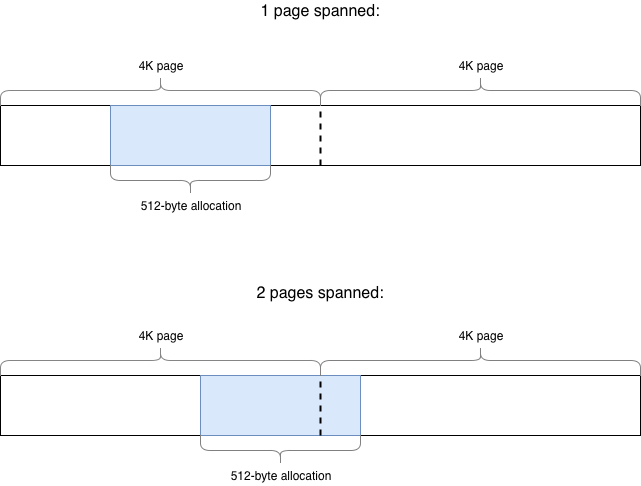
\includegraphics[width=\textwidth]{diagrams/allocation_spanned_pages.png}
	\label{fig:allocation-spanned-pages}
	\caption{A memory allocation can span different number of pages depending on where it begins}
\end{figure}

\subsection{Handling re-allocations}

Handling \lstinline!realloc()! is a combination of a deallocation and an allocation, with a couple of tweaks. I will present the logic here in the conceptual level, as the Dangless-specific technical details of it are the same as with allocations and deallocations already covered previously.

First, the call \lstinline!realloc(NULL, some_size)! is valid according to the standard and is equivalent to \lstinline!malloc(some_size)!. Second, we have to be able to handle the unusual case when the original pointer did not originate from Dangless, but directly from the system allocator: this can happen for instance if the original allocation occurred before Dangless was initialized. We deal with both of these cases by treating them the same way as a \lstinline!malloc()! call: simply allocate some new virtual memory to remap the system allocator's result to.

Finally, we want to perform the reallocation in-place when possible: that is, re-use the same remapped virtual memory region. There are 3 cases to consider with regards to how the number of pages spanned by the allocation changes:

\begin{enumerate}
	\item Stays the same: nothing to do.
	\item Decreases, i.e. the new size is less than the old size such that the allocation is now held by fewer pages than before: invalidate the pages that were cut off, in the same way as we would handle a deallocation.
	\item Increases, i.e. the new size is greater than the old size such that the allocation is now held by more pages than before: allocate a new virtual memory region large enough to fit the new allocation size, and invalidate the entire old region. This could potentially be optimized: if the virtual memory allocator owns the pages that are directly after the old virtual memory region (ensuring that these pages are not in use nor have they been invalidated before), then we could simply grow our virtual memory region in-place.
\end{enumerate}

It's worth noting that if the system allocator was unable to perform the reallocation in-place, that does not mean that we can't perform our work in-place: in this case it's sufficient if we just update the physical memory addresses of the original virtual memory region and flush the corresponding TLB entries. However, this optimization is not currently implemented in Dangless.

\section{Fixing up vmcalls}
\label{sec:vmcall-pointer-rewriting}

\subsection{The problem}

One of the goals of Dune is to remain as simple as possible, and not re-implement most functionality of operating system kernels when not absolutely necessary. This means that most system calls performed by the application running inside Dune are not actually handled by Dune itself, but rather are passed on to the host kernel via the \lstinline!vmcall! instruction. (\lstinline!vmcall! is identical to \lstinline!syscall!, except it exits the virtual environment first.) This includes tasks as common as I/O operations (such as \lstinline!printf()! or \lstinline!fopen()!), or even memory management (such as \lstinline!mmap()!).

This presents a challenge for Dangless, which can be efficient because it can directly manipulate the page tables inside the virtual environment (guest machine) itself, without having to manipulate the host's page tables (which would only be possible via a system call such as \lstinline!mprotect()!). However, any virtual memory addresses returned from Dangless will only be valid inside the guest environment, meaning that attempting to pass such a memory address to the host kernel when performing a system call (vmcall) will fail with \lstinline!EINVAL!.

To demonstrate the problem, first consider the following:

\begin{lstlisting}
puts("Hello world!\n");
\end{lstlisting}

The \lstinline!puts()! standard library function used here is a comparatively simple wrapper around the \lstinline!write()! system call, and unlike \lstinline!printf()!, does not perform any formatting or other manipulation of the string~\cite{glibc-puts-analysis}. Recall that in C, strings are represented by null-terminated character arrays, and are typically passed to functions as \lstinline!const char*!: a (virtual) memory address pointing to the first character of the string. Since in this example, the argument to \lstinline!puts()! is a string literal, the string data is stored in the executable's data section (such as \texttt{.rodata}) without any dynamic memory allocation that would go through Dangless. The result is that the pointer passed to the \lstinline!write()! vmcall references virtual memory that is mapped by the host machine, so the call will succeed.

\begin{lstlisting}
void determineAnswer(char* buffer) {
	strcpy(buffer, "Fourty-two");
}

char* answerBuffer = malloc(64 * sizeof(char));
determineAnswer(answerBuffer);

puts("The answer is: ");
puts(answerBuffer);
puts("\n");

free(answerBuffer);
\end{lstlisting}

The problem here is that we are passing a \lstinline!malloc()!-d buffer to \lstinline!puts()!. Since \lstinline!malloc()! refers to \lstinline!dangless_malloc()!, it will perform virtual memory remapping inside the guest system, yielding a pointer value in \lstinline!answer! that is valid inside the guest machine, but not in the host machine. (Of course, the data is present in the host physical memory, but is not mapped to host virtual memory.) The \lstinline!write()! system call when executed by the host, is not going to be amused by this fact, and is going to return the error code \texttt{EINVAL}, indicating an invalid argument.

In this case by knowing how Dangless works it is easy to spot the problem. However, often dynamic memory allocation is performed and the resulting pointer is passed to a system call in a way that's not immediately obvious from the user code, such as when done internally by the standard library implementation. The simplest example is probably \lstinline!printf()!, which can call \lstinline!malloc()! in some circumstances~\cite{glibc-printf-malloc}~\cite{glibc-printf-malloc-vulnerability}. I've also already mentioned how \lstinline!dlsym()! when running for the first time will call \lstinline!calloc()!.

\subsection{Intercepting vmcalls}

In order to fix this problem, Dangless needs to intercept any system calls that are about to be forwarded to the host kernel. This capability is not provided by default in Dune, so I've implemented it (\texttt{dune-ix-vmcallhooks.patch}), allowing Dangless to register a pre- and post-hook function that will be called before and after a \lstinline!vmcall! instruction is performed by Dune, respectively. In the pre-hook, Dangless can access and modify the system call number, any of the arguments, and even the return address. Similarly, the post-hook exposes the syscall return code.

\subsection{Determining which arguments to rewrite}

The next problem is how to determine what the system call arguments are, and which of them can possibly reference a Dangless-remapped pointer. Note that it is not sufficient to find the pointers among the arguments themselves, as pointers can be nested: the arguments can be pointers to arrays or structures which in turn contain pointers -- sometimes, after a few layers of indirection. Examples include the \lstinline!readv()! and \lstinline!writev()! system calls, which are used by GNU implementation of the \lstinline!<iostream>! standard C++ header such as when writing to \lstinline!std::cout!, i.e. \lstinline!stdout!:

\begin{lstlisting}
ssize_t readv (int fd, const struct iovec *v, int n);
ssize_t writev(int fd, const struct iovec *v, int n);

struct iovec {
	void  *iov_base; /* Starting address */
	size_t iov_len;  /* Number of bytes */
};
\end{lstlisting}

When handling either of these functions, not just the \lstinline!const struct iovec *v! pointer has to be fixed, but also the \lstinline!void *iov_base! pointer inside the pointer \lstinline!struct iovec!.

Another example is the functions \lstinline!execve()! and \lstinline!execveat()!:

\begin{lstlisting}
int execve(const char *filename, char *const argv[], char *const envp[]);
int execveat(int dirfd, const char *pathname, char *const argv[], char *const envp[], int flags);
\end{lstlisting}

Besides the \lstinline!const char *filename! simple pointer, the parameters \lstinline!char *const argv[]! and \lstinline!char *const envp[]! are both a null-terminated array of pointers, in which every entry has to be fixed.

Finally, pointers to more complicated structures are also sometimes passed as system call arguments:

\begin{lstlisting}
ssize_t recvmsg(int sockfd, struct msghdr *msg, int flags);

struct msghdr {
	void         *msg_name;       /* optional address */
	socklen_t     msg_namelen;    /* size of address */
	struct iovec *msg_iov;        /* scatter/gather array */
	size_t        msg_iovlen;     /* # elements in msg_iov */
	void         *msg_control;    /* ancillary data, see below */
	size_t        msg_controllen; /* ancillary data buffer len */
	int           msg_flags;      /* flags on received message */
};
\end{lstlisting}

So, we need some way to determine which arguments of the system call can be a pointer, and identify what data structure it points to in order to find any nested pointers. Essentially, what we need is to be able to tell for a system call number what arguments it takes and what type they are. For this purpose, I have created a Python module \texttt{linux-syscallmd} (source on GitHub~\cite{github-linux-syscallmd}) that parses the Linux kernel header file \texttt{include/linux/syscalls.h} and exposes system call metadata to user code. The Dangless script at \texttt{make/gen\_vmcall\_fixup\_info.py} then uses this information to generate a file containing C code that can be \lstinline!#include!-d to utilize this data inside Dangless:

\begin{lstlisting}
// sources/src/platform/dune/vmcall_fixup_info.h

enum vmcall_param_fixup_type {
	VMCALL_PARAM_NONE,
	VMCALL_PARAM_FLAT_PTR,
	VMCALL_PARAM_IOVEC,
	VMCALL_PARAM_PTR_PTR,
	VMCALL_PARAM_MSGHDR
}

struct vmcall_param_fixup_info {
	enum vmcall_param_fixup_type fixup_type;
};

struct vmcall_fixup_info {
	i8 num_params;
	struct vmcall_param_fixup_info params[SYSCALL_MAX_ARGS];
};

// sources/src/platform/dune/vmcall_fixup_info.c

static const struct vmcall_fixup_info g_vmcall_fixup_info_table[] = {
	// generated by make/gen_vmcall_fixup_info.py
	#include "dangless/build/common/vmcall_fixup_info.inc"
};
\end{lstlisting}

The generated array is indexed by the number of a system call to find its corresponding entry. Then we can iterate through the arguments and act on them based on the \lstinline!enum vmcall_param_fixup_type! value.

As an example, the entry for the \lstinline!clone()! system call looks like this:

\begin{lstlisting}
static const struct vmcall_fixup_info s_clone_info = {
	.num_params = 5,
	.params = {
		// unsigned long flags
		[0] = {
			.fixup_type = VMCALL_PARAM_NONE
		},
		
		// void *child_stack
		[1] = {
			.fixup_type = VMCALL_PARAM_FLAT_PTR
		},
		
		// int *ptid
		[2] = {
			.fixup_type = VMCALL_PARAM_FLAT_PTR
		},
		
		// int *ctid
		[3] = {
			.fixup_type = VMCALL_PARAM_FLAT_PTR
		},
		
		// unsigned long newtls
		[4] = {
			.fixup_type = VMCALL_PARAM_NONE
		}
	}
};
\end{lstlisting}

\subsection{Rewriting the pointers}

Now that we know which arguments to rewrite or "fix-up", we can use the same logic as \lstinline!dangless_free()! to get the canonical pointer from a potentially-remapped one (see Section~\ref{ssec:deallocations}). We then replace the remapped pointer value with the canonical one in the system call arguments.

In case of nested pointers this involves modifying the referenced in-memory data, meaning we cannot simply replace the pointer. This is because the original pointer was a remapped pointer, allocated via Dangless, and will be deallocated via Dangless. However, due to the nested pointer fix-up, the user code can now potentially access the canonical (non-remapped) pointer, opening the door to dangling pointer errors. Furthermore, should a canonical pointer be passed to \lstinline!dangless_free()!, it cannot invalidate the remapped memory region as it doesn't know where it might be.

To demonstrate, consider the following code:

\begin{lstlisting}
char *first = malloc(32);
strcpy(first, "Hello ");

char *second = malloc(32);
strcpy(second, "world!");

struct iovec iov[2];
iov[0].iov_base = first;
iov[0].iov_len = strlen(first);
iov[1].iov_base = second;
iov[1].iov_len = strlen(second);

writev(STDOUT_FILENO, iov, 2);
\end{lstlisting}

Due to pointer rewriting the system call succeeds, but afterwards we end up with \lstinline|iov[0].iov_base != first| and \lstinline|iov[1].iov_base != second|, as they have been replaced by their canonical counterparts to make the system call succeed on the host kernel.

Later, we deallocate the buffers:

\begin{lstlisting}
free(second);
free(first);
\end{lstlisting}

This is fine, since the \lstinline!first! and \lstinline!second! variables were not affected by the pointer rewriting, so Dangless correctly invalidates the remapped regions in \lstinline!dangless_free()!. But then, later:

\begin{lstlisting}
fprintf(stderr, "Attempted writev() with '%s' and '%s'!\n", iov[0].iov_base, iov[1].iov_base);
\end{lstlisting}

Here we have an attempted memory access through two dangling pointers. Recall that, due to pointer rewriting, \lstinline|iov[0].iov_base| and \lstinline|iov[1].iov_base| are the canonical pointers (as returned by \lstinline!sysmalloc()!) and so do not point into the remapped region that was invalidated by the earlier \lstinline!dangless_free()! calls. Therefore, this error will not be caught by Dangless!

To resolve this situation, for every nested pointer fix-up, Dangless records the pointer location (a pointer to the user pointer) as well as the original value stored there (the Dangless-remapped pointer value) in a buffer. After the vmcall returns but before it jumps back into user code, we then go through the records and restore any such rewritten pointer values to their original ones, preventing the user from being exposed to non-remapped pointer values.

\subsection{Limitations}

This approach is limited in that Dangless can only handle system calls, arguments, and argument types that \texttt{linux-syscallmd} recognizes when building Dangless.

For instance, \texttt{linux-syscallmd} currently does not understand or process preprocessor macros, such as \lstinline!#if! and \lstinline!#ifdef! sections. This means that system call signatures not relevant for the current system will also be parsed, leading to conflicting signatures for some system calls, such as \lstinline!clone()!. \texttt{linux-syscallmd} currently does not handle this situation, and will just pick the last occurrence of the same system call in the source file, which may be different than the signature actually used by the kernel. Because of this, Dangless has special handling of the \lstinline!clone()! system call, but naturally that can't extend to e.g. system calls introduced in the future.

As of writing, I do not know of a better way to approach this. Fixing the present limitation would involve knowing what values were used for each preprocessor macro while building the kernel, and I'm not aware of any way in which the kernel exposes this information.

Another issue is understanding which arguments can hold pointer or nested pointer values. For the vast majority of system calls this is straight-forward, as \texttt{linux/syscall.h} consistently marks the pointer arguments as \lstinline!__user *!, and the pointed type is obvious, whether it's \lstinline!char! or \lstinline!struct iovec!. But some system calls will interpret the same argument differently depending on the context of the call, such as \lstinline!ptrace()!. The signature of \lstinline!ptrade()! is as follows:

\begin{lstlisting}
long ptrace(enum __ptrace_request request, pid_t pid, void *addr, void *data);
\end{lstlisting}

Notice that \lstinline!addr! and \lstinline!data! are both untyped (\lstinline!void!) pointers. How they are interpreted differs depending on the value of the \lstinline!request! argument. Some examples:

\begin{itemize}
	\item \lstinline!PTRACE_TRACEME!: both \lstinline!addr! and \lstinline!data! are ignored.
	\item \lstinline!PTRACE_PEEKTEXT!: \lstinline!addr! does \emph{not} correspond to pointer in the address space of the caller, but rather, refers to a location in the address space of the target application. The same pointer value may reference a memory region that's unmapped, or worse, mapped for something completely different in the address space of the calling process. As such, Dangless should not touch it. \lstinline!data! is ignored.
	\item \lstinline!PTRACE_POKEDATA!: \lstinline!addr! refers to a memory address in the target process. \lstinline!data! might not be a pointer value at all, but rather the word to be copied into the target process' memory.
	\item \lstinline!PTRACE_GETREGS!: \lstinline!data! is an actual pointer in the calling process, while \lstinline!addr! is ignored.
	\item \lstinline!PTRACE_GETREGSET!: \lstinline!addr! is not a pointer value at all, but rather an enumeration. \lstinline!data! is an actual pointer to the calling process' memory, but it references a \lstinline!struct iovec! value, meaning that it will contain nested pointers that also have to be fixed up by Dangless.
\end{itemize}

\lstinline!ptrace()! is a special case due to its very specialized nature, and it's unlikely to be used at all in the vast majority of applications that Dangless would be relevant for. Because of this Dangless ignores \lstinline!ptrace()!, even though it would be possible to cover all of these scenarios.

There may be other system calls that have similar behaviour, although likely not as pathological as \lstinline!ptrace()!. These are currently not handled in any way by texttt{linux-syscallmd} nor Dangless. Supporting all of these scenarios would inevitably involve extending Dangless to handle each on a case-by-case basis.
